\documentclass{beamer}
\mode<presentation>
\usepackage{amsmath}
\usepackage{amssymb}
%\usepackage{advdate}
\usepackage{graphicx}
\usepackage{adjustbox}
\usepackage{subcaption}
\usepackage{enumitem}
\usepackage{multicol}
\usepackage{mathtools}
\usepackage{listings}
\usepackage{url}
\def\UrlBreaks{\do\/\do-}
\usetheme{Boadilla}
\usecolortheme{lily}
\let\vec\mathbf
\setbeamertemplate{footline}
{
  \leavevmode%
  \hbox{%
  \begin{beamercolorbox}[wd=\paperwidth,ht=2.25ex,dp=1ex,right]{author in head/foot}%
    \insertframenumber{} / \inserttotalframenumber\hspace*{2ex} 
  \end{beamercolorbox}}%
  \vskip0pt%
}
\setbeamertemplate{navigation symbols}{}

\providecommand{\nCr}[2]{\,^{#1}C_{#2}} % nCr
\providecommand{\nPr}[2]{\,^{#1}P_{#2}} % nPr
\providecommand{\mbf}{\mathbf}
\providecommand{\pr}[1]{\ensuremath{\Pr\left(#1\right)}}
\providecommand{\qfunc}[1]{\ensuremath{Q\left(#1\right)}}
\providecommand{\sbrak}[1]{\ensuremath{{}\left[#1\right]}}
\providecommand{\lsbrak}[1]{\ensuremath{{}\left[#1\right.}}
\providecommand{\rsbrak}[1]{\ensuremath{{}\left.#1\right]}}
\providecommand{\brak}[1]{\ensuremath{\left(#1\right)}}
\providecommand{\lbrak}[1]{\ensuremath{\left(#1\right.}}
\providecommand{\rbrak}[1]{\ensuremath{\left.#1\right)}}
\providecommand{\cbrak}[1]{\ensuremath{\left\{#1\right\}}}
\providecommand{\lcbrak}[1]{\ensuremath{\left\{#1\right.}}
\providecommand{\rcbrak}[1]{\ensuremath{\left.#1\right\}}}
\theoremstyle{remark}
\newtheorem{rem}{Remark}
\newcommand{\sgn}{\mathop{\mathrm{sgn}}}
\providecommand{\abs}[1]{\vert#1\vert}
\providecommand{\res}[1]{\Res\displaylimits_{#1}} 
\providecommand{\norm}[1]{\lVert#1\rVert}
\providecommand{\mtx}[1]{\mathbf{#1}}
\providecommand{\mean}[1]{E[ #1 ]}
\providecommand{\fourier}{\overset{\mathcal{F}}{ \rightleftharpoons}}
%\providecommand{\hilbert}{\overset{\mathcal{H}}{ \rightleftharpoons}}
\providecommand{\system}[1]{\overset{\mathcal{#1}}{ \longleftrightarrow}}
%\providecommand{\system}{\overset{\mathcal{H}}{ \longleftrightarrow}}
	%\newcommand{\solution}[2]{\vec{Solution:}{#1}}
%\newcommand{\solution}{\noindent \vec{Solution: }}
\providecommand{\dec}[2]{\ensuremath{\overset{#1}{\underset{#2}{\gtrless}}}}
\newcommand{\myvec}[1]{\ensuremath{\begin{pmatrix}#1\end{pmatrix}}}


\lstset{
%language=C,
frame=single, 
breaklines=true,
columns=fullflexible
}
\lstset{
  language=C,
  basicstyle=\ttfamily\footnotesize,
  keywordstyle=\color{blue}\bfseries,
  commentstyle=\color{gray}\itshape,
  stringstyle=\color{orange},
  numbers=left,
  numberstyle=\tiny\color{gray},
  breaklines=true,
  frame=single,
  showstringspaces=false,
  tabsize=4,
  captionpos=b
}
\numberwithin{equation}{section}
\lstset{
  language=Python,
  basicstyle=\ttfamily\small,
  keywordstyle=\color{blue},
  stringstyle=\color{orange},
  numbers=left,
  numberstyle=\tiny\color{gray},
  breaklines=true,
  showstringspaces=false
}

\title{Problem 2.10.24}
\author{Sujal Rajani}

\date{\today} 
\begin{document}

\begin{frame}
\titlepage
\end{frame}


\section{Question}
\begin{frame}{Question}
\textbf{Question}:
 \noindent  Let $\vec{x}$,$\vec{y}$ and $\vec{z}$ be three vectors each of magnitude $\sqrt 2$ and the angle between each pair of them is $\dfrac{\pi}{3}$. If $\vec{a}$ is a non-zero vector perpendicular to $\vec{x}$ and $\vec{y}$ x $\vec{z}$ and $\vec{b}$ is a non-zero vector perpendicular to $\vec{y}$ and $\vec{z}$ x $\vec{x}$, then
 
 
  (A) $\vec{b}$ = ($\vec{b}\cdot\vec{z}$)($\vec{z}-\vec{x}$)
  \\
(B) $\vec{a}$ = ($\vec{a}.\vec{y}$)($\vec{y}-\vec{z}$)
 \\
 (C)$\vec{a}.\vec{b}$ = -($\vec{a}.\vec{y}$)($\vec{b}.\vec{z}$)
 \\
 (D)$\vec{a}$ = -($\vec{a}.\vec{y}$)($\vec{z}-\vec{y}$)
 
 
\end{frame}
\begin{frame}{Solution}
\textbf{Solution:} 
as mentioned in the question : 
\begin{align*}
    ||\vec{x}||=\sqrt{2},
    ||\vec{y}||=\sqrt{2},
    ||\vec{z}||=\sqrt{2}
    \end{align*}
    \begin{equation}
\vec{x}^\top\vec{y}=1,\vec{x}^\top\vec{z}=1,\vec{y}^\top\vec{z}=1
\end{equation}

\end{frame}
\begin{frame}{Solution}
If $\vec{a}$ is a non-zero vector perpendicular to $\vec{x}$ and $\vec{y}$ x $\vec{z}$ this implies :
\\
\begin{align*}
    \vec{a}^\top\vec{x}=0, \vec{a}^\top(\vec{y} X \vec{z})=0
\end{align*}


this implies that  $\vec{x}$ and $\vec{y} X \vec{z}$ lie in the same plane and their vector product is parallel to $\vec{a}$
\\
so the vector product of 
\\
\begin{align*}
    \vec{a}X(\vec{x}X(\vec{y} X \vec{z}))=0
\end{align*}
\end{frame}
\begin{frame}{vector product}
defining : triple vector product 
\begin{align*}
    (\vec{x}X(\vec{y} X \vec{z}))=(\vec{x}^\top \vec{z})\vec{y}-(\vec{x}^\top \vec{y})\vec{z}
\end{align*}
\end{frame}
\begin{frame}{Solution}
by equation (1.1) : $\vec{x}^\top\vec{z}=1,\vec{x}^\top\vec{y}=1$
\begin{align*}
    \vec{a}X(\vec{x}X(\vec{y} X \vec{z}))=(\vec{x}^\top\vec{z})(\vec{y}X\vec{a})-(\vec{x}^\top\vec{y})(\vec{z}X\vec{a)}=\vec{a}X(\vec{y}-\vec{z})=0
\end{align*}
as $\vec{a}$ is parallel to $\vec{y}-\vec{z}$ so we can say that :
\begin{align*}
    \vec{a}=k(\vec{y}-\vec{z})
\end{align*}    
k is a  constant
\end{frame}
\begin{frame}{Solution}
If $\vec{b}$ is a non-zero vector perpendicular to $\vec{y}$ and $\vec{z}$ x $\vec{x}$ this implies :
\\
\begin{align*}
    \vec{b}^\top\vec{y}=0, \vec{b}^\top(\vec{z} X \vec{x})=0
\end{align*}
this implies that  $\vec{x}$ and $\vec{y} X \vec{z}$ lie in the same plane and their vector product is parallel to $\vec{a}$
\\
so the vector product of 
\\
\begin{align*}
    \vec{b}X(\vec{y}X(\vec{z} X \vec{x}))=0
\end{align*}
\end{frame}
\begin{frame}{Solution}
by equation (1.1) :  $\vec{x}^\top\vec{y}=1,\vec{z}^\top\vec{y}=1$
\begin{align*}
    \vec{bX}(\vec{y}X(\vec{z} X \vec{x}))=(\vec{y}^\top\vec{x})(\vec{z}X\vec{b})-(\vec{y}^\top\vec{z})(\vec{x}X\vec{b})=\vec{b}X(\vec{z}-\vec{x})=0 
\end{align*}
as $\vec{b}$ is parallel to $\vec{z}-\vec{x}$ so we can say that :
\begin{align*}
    \vec{b}=m(\vec{z}-\vec{x}) 
\end{align*}
m is a  constant
\end{frame}
\begin{frame}{Solution}
now we check options one by one :
\\
\\
option (a)
\\
$\vec{b}$ = ($\vec{b}.\vec{z}$)($\vec{z}-\vec{x}$)
\\
we are putting b on both sides=
 \begin{align*}
    m(\vec{z}-\vec{x})=( m(\vec{z}-\vec{x})^\top\vec{z})(\vec{z}-\vec{x}) 
    \\
    m(\vec{z}-\vec{x})=m(\vec{z}.\vec{z}-\vec{x}^\top\vec{z})(\vec{z}-\vec{x}) 
    \\
     m(\vec{z}-\vec{x})= m(\vec{z}-\vec{x})
 \end{align*}
 option A is correct . 
\end{frame}
\begin{frame}{Solution}
 option (b)
\\
$\vec{a}$ = ($\vec{a}^\top\vec{y}$)($\vec{y}-\vec{z}$)
\\
we are putting a on both sides=
\\
 \begin{align*}
   k(\vec{y}-\vec{z})=(k(\vec{y}-\vec{z})^\top\vec{y})(\vec{y}-\vec{z})
    \\
    k(\vec{y}-\vec{z})=(k(\vec{y}^\top\vec{y}-\vec{y}^\top\vec{z})(\vec{y}-\vec{z})
    \\
    \\
     k(\vec{y}-\vec{z})= k(\vec{y}-\vec{z})
 \end{align*}
 option B is correct .
\end{frame}
\begin{frame}{Solution}
 option (c)
\\
$\vec{a}^\top\vec{b}$ = -($\vec{a}^\top\vec{y}$)($\vec{b}^\top\vec{z}$)
\\
we are putting a and b on both sides=
\\
\begin{align*}
    k(\vec{y}-\vec{z})m(\vec{z}-\vec{x})=-( m(\vec{z}-\vec{x}).\vec{z})(k(\vec{y}-\vec{z})^\top\vec{y})
    \\
    -km=-km
\end{align*}
option C is correct  .
\\
option D is correct because option B is correct.
\end{frame}
\begin{frame}{Solution}

\\
for plotting we are assuming the position vector :
\begin{align*}
    \vec x=\myvec{1\\1\\0},\vec y=\myvec{1\\0\\1},\vec z=\myvec{0\\1\\1},\vec a=\myvec{-1\\1\\0},\vec b=\myvec{-1\\0\\1}
\end{align*}
\end{frame}
\begin{frame}{fragile}
 \begin{figure}[H]
    \centering
    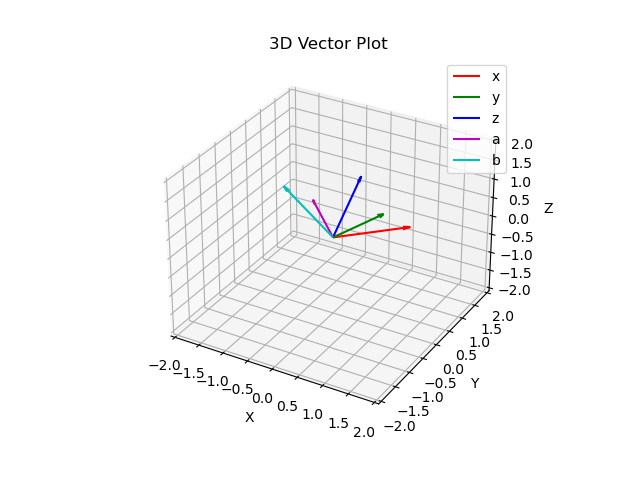
\includegraphics[width = 0.7\columnwidth]{../figs/img.png}
    \caption*{}
    \label{figs}
\end{figure}
\end{frame}
\begin{frame}[fragile]
\frametitle{C Code }
\begin{lstlisting}[language=C]
#include <stdio.h>
#include <math.h>

// Vector operations
typedef struct {
    double x, y, z;
} Vector;

Vector add(Vector a, Vector b) {
    return (Vector){a.x + b.x, a.y + b.y, a.z + b.z};
}

\end{lstlisting}
\end{frame}

\begin{frame}[fragile]
\frametitle{C Code }
\begin{lstlisting}[language=C]
 Vector sub(Vector a, Vector b) {
    return (Vector){a.x - b.x, a.y - b.y, a.z - b.z};
}

Vector scalarMul(double c, Vector a) {
    return (Vector){c * a.x, c * a.y, c * a.z};
}

double dot(Vector a, Vector b) {
    return a.x*b.x + a.y*b.y + a.z*b.z;
}


    
\end{lstlisting}
\end{frame}
\begin{frame}[fragile]
\frametitle{C Code }
\begin{lstlisting}[language=C]
Vector cross(Vector a, Vector b) {
    return (Vector){
        a.y*b.z - a.z*b.y,
        a.z*b.x - a.x*b.z,
        a.x*b.y - a.y*b.x
    };
}

void printVec(Vector v) {
    printf("(%.2f, %.2f, %.2f)", v.x, v.y, v.z);
}

\end{lstlisting}
\end{frame}
\begin{frame}[fragile]
\frametitle{C Code }
\begin{lstlisting}[language=C]
int main() {
    // Define x, y, z such that |x|=|y|=|z|=sqrt(2) and angle = 60 deg
    // Example choice:
    Vector x = {1, 1, 0};   // |x| = sqrt(2)
    Vector y = {1, 0, 1};   // |y| = sqrt(2)
    Vector z = {0, 1, 1};   // |z| = sqrt(2)
    // These satisfy x·y = x·z = y·z = 1 → cosθ = 1/2 → θ = 60°

    // Define a ⟂ x, y, x×z → take a = cross(x, y)
    Vector a = cross(x, y);

    // Define b ⟂ y, z, z×x → take b = cross(y, z);

    Vector b = cross(y, z);

\end{lstlisting}
\end{frame}
\begin{frame}[fragile]
\frametitle{C Code }
\begin{lstlisting}[language=C]
  printf("x = "); printVec(x); printf("\n");
    printf("y = "); printVec(y); printf("\n");
    printf("z = "); printVec(z); printf("\n");

    printf("a = "); printVec(a); printf("\n");
    printf("b = "); printVec(b); printf("\n\n");

    // Now check conditions
    Vector lhs1 = b;
    Vector rhs1 = scalarMul(dot(b, z), sub(z, x));
    printf("1) b == (b.z)(z - x) ? -> (%f,%f,%f)\n", lhs1.x-rhs1.x, lhs1.y-rhs1.y, lhs1.z-rhs1.z);

\end{lstlisting}
\end{frame}
\begin{frame}[fragile]
\frametitle{C Code }
\begin{lstlisting}[language=C]
   Vector lhs2 = a;
    Vector rhs2 = scalarMul(dot(a, y), sub(y, z));
    printf("2) a == (a.y)(y - z) ? -> (%f,%f,%f)\n", lhs2.x-rhs2.x, lhs2.y-rhs2.y, lhs2.z-rhs2.z);

    double lhs3 = dot(a, b);
    double rhs3 = -(dot(a, y) * dot(b, z));
    printf("3) a·b == -(a.y)(b.z) ? -> LHS=%.2f, RHS=%.2f\n", lhs3, rhs3);

\end{lstlisting}
\end{frame}
\begin{frame}[fragile]
\frametitle{C Code }
\begin{lstlisting}[language=C]
  Vector lhs4 = a;
    Vector rhs4 = scalarMul(-(dot(a, y)), sub(z, y));
    printf("4) a == -(a.y)(z - y) ? -> (%f,%f,%f)\n", lhs4.x-rhs4.x, lhs4.y-rhs4.y, lhs4.z-rhs4.z);

    return 0;
}
\end{lstlisting}
\end{frame}

\section{Python Code}
\begin{frame}[fragile]
\frametitle{Python Code for Plotting}
\begin{lstlisting}[language=Python]
import numpy as np
import matplotlib.pyplot as plt
import matplotlib as mp
mp.use("TkAgg")

# ------------------------
# Step 1: Define vectors
# ------------------------
vectors = {
    "x": np.array([1, 1, 0]),
    "y": np.array([1, 0, 1]),
    "z": np.array([0, 1, 1]),
    "a": np.array([-1, 1, 0]),
    "b": np.array([-1, 0, 1])
}

\end{lstlisting}

\end{frame}
\begin{frame}[fragile]
\frametitle{Python Code for Plotting}
\begin{lstlisting}[language=Python]
colors = {
    "x": "red",
    "y": "blue",
    "z": "green",
    "a": "orange",
    "b": "purple"
}

# ------------------------
# Step 2: Plot vectors
# ------------------------
fig = plt.figure(figsize=(8, 8))
ax = fig.add_subplot(111, projection="3d")
for name, vec in vectors.items():
    ax.quiver(0, 0, 0, vec[0], vec[1], vec[2],
              color=colors[name], linewidth=2, arrow_length_ratio=0.1, label=name)

\end{lstlisting}

\end{frame}
\begin{frame}[fragile]
\frametitle{Python Code for Plotting}
\begin{lstlisting}[language=Python]

# Step 3: Formatting
# ------------------------
ax.set_xlim([-2, 2])
ax.set_ylim([-2, 2])
ax.set_zlim([-2, 2])

ax.set_xlabel("X-axis")
ax.set_ylabel("Y-axis")
ax.set_zlabel("Z-axis")
ax.set_title("3D Vector Plot")
ax.legend()

plt.show()

\end{lstlisting}

\end{frame}

\end{document}